\chapter{Implementacija}
\section{Korištene tehnologije}

\subsection{Spring Boot}
Za razvoj backenda web aplikacije "Vožnja +" izabran je Spring Boot razvojni okvir koji znatno pojednostavljuje i olakšava razvoj aplikacija u Programskom jeziku Java. Glavna prednost Spring Boota je smanjena konfiguracijska složenost i ubrzan razvoj aplikacije. Razvoj aplikacije započeo je upotrebom Spring inicijalizatora projekta na kojem se odabire projekt (Maven), programski jezik (Java) i verzija Spring Boota. Pri inicijalizaciji dodaju se potrebne ovisnosti koje se kasnije po potrebi nadograđuju u pom.xml datoteci. Osnovne konfiguracijske postavke definiraju se u datoteci application.properties.  U razvoju aplikacije ključnu ulogu igraju anotacije koje omogućuju konfiguraciju i upravljanje komponentama bez potrebne za opsežnim XML konfiguracijama. Primjerice, anotacija @Autowired koristi se za automatsku injekciju zavisnosti koja eliminira potrebu za ručnom konfiguracijom. To znači da umjesto ručnog konfiguriranja komponente pri svakom njenom korištenju, sve što trebamo napraviti je iznad instanciranja komponente dodati spomenutu anotaciju. Ostatak anotacija bit će objašnjeni u poglavlju "Poslužitelj" gdje će se detaljnije objasniti  implementacija poslužiteljske strane i korištenje karakterističnih Spring Boot anotacija. Korišteni radni okvir je IntelliJ.
\subsection{React}
Za razvoj frontenda korišten je skriptni jezik JavaScript koji se izvršava u web pregledniku korisnika web aplikacije. Za razvoj korisničkih sučelja korištena je Raect razvojna biblioteka. React je biblioteka otvorenog koda temeljena na komponentama koje se koriste s izgradnju sučelja. Svaka komponenta ima mogućnost održavanja svog stanja i komponiranja u složenije dijelove grafičkog sučelja. Glavna karakteristika Reacta je njegov dizajn koji omogućava ponovno renderiranje komponente tek pri promjeni podataka što je učinkovitije nego ponovno renderiranje cijele stranice. Pored Reacta, za učinkovit razvoj korisničkih sučelja korištena je  Chakra UI biblioteka komponenti koja pruža polu-gotove gradivne blokove za izgradnju aplikacije. Svaki gradivni element prilagođen je svojoj namjerni kako bi se osiguralo što bolje korisničko iskustvo. Korišteni radni okvir je Visual Studio Code.

\subsection{Cloudinary}
Za skladištenje i manipulaciju medijskim sadržajem u aplikaciji korištena je Cloudinary platforma kojoj se pristupa pomoću API-ja (engl. application programming interface). Glavne funkcionalnosti Cloudinary platforme koje su korištene za aplikaciju su skladištenje i dohvat fotografija. Platforma osigurava sigurnost i podržava kontroliran pristup budući da se pri konfiguraciji servisa koriste Cloud name (ime oblaka), API key (API ključ) i API secret (API tajna) koji se provjeravaju pri svakom pristupu.

\subsection{EmailJS}
Integracija s Gmail servisom ostvarena je pomoću EmailJS servisa koji omogućava direktno slanje emailova iz JavaScript aplikacija bez potrebe za poslužiteljem. Na ovaj način omogućeno je učinkovito slanje mailova direktno iz aplikacije. Nakon konfiguracije, servis brine o komunikaciji i autentificiranom pristupu svojim uslugama.

\section{Dijagram razmještaja sustava}
Na slici 4.1. možemo vidjeti dijagram razmještaja sustava. Za arhitekturu odabrana je arhitektura poznata po nazivu "klijent-poslužitelj". Glavna karakteristika spomenute arhitekture je razdvojenog funkcionalnosti na usluge koje pruža poslužitelj i usluge koje pruža klijent. Korisnici web aplikacije pristupaju aplikaciji putem web preglednika na vlastitom računalu. Korisničko računalo ima ulogu klijenta koje u ime korisnika obavlja zahtjeve prema poslužitelju. Web poslužitelj i poslužitelj baze podataka nalaze se na zasebnom računalu. Interakcija između korisničkog i poslužiteljskog računala odvija se putem HTTP (HyperText Transfer Protocol) protokola. Osnovne karakteristike HTTP protokola su komunikacija putem zahtjeva i odgovora te neovisnost novog zahtjeva o prethodno poslanim zahtjevima. 

\begin{figure}[H]
					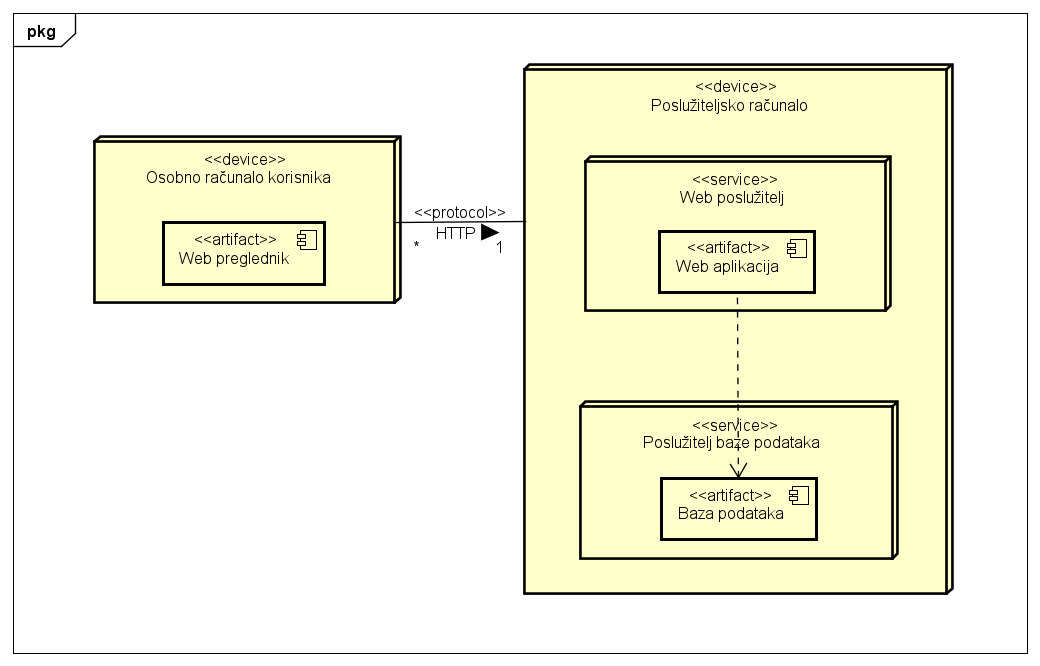
\includegraphics[width=\textwidth]{slike/DeploymentDiagram.png} 
					\centering
					\caption{Dijagram razmještaja sustava}
					\label{fig:promjene}
				\end{figure}
\subsection{Klijent}
Klijentska strana  zasnovana je na funkcijskim komponentama pomoću kojih se gradi izgled cijele aplikacije. React koristi virtualni DOM (engl. Data Object Model) za poboljšanje svojih performansi. Kada se stanje aplikacije promijeni, React prvo ažurira virtualni DOM koji onda uspoređuje s pravim modelom kako bi minimalno ažurirao stvarni model. App.js je ključna komponenta u kojoj su definirane korisničke rute i komponente koje se koriste za izgradnju pojedinih sučelja. Sučelje koje se prikazuje korisniku ovisi u njegovoj ulozi koja se sprema u memoriju sjednice. Svaka komponenta ima svoje unutarnje stanje koje određuje kako se komponenta prikazuje i ponaša. Za očuvanje stanja i ažuriranje komponenti koriste se dvije posebne funkcionalnosti Reacta: useState i useEffect hook-ovi. Hook-ovi služe za baratanje s popratnim efektima pojedine komponente. useState hook služi za održavanje lokalnog stanja funkcijskim komponentama, a useEffect hook služi za ažuriranje komponente, odnosno njenih podataka. Kako bi se moglo navigirati između različitih komponenti, korišten je React Router koji omogućava definiranje višestrukih ruta unutar aplikacije.

\subsection{Poslužitelj}
Aplikacija je izgrađena korištenjem objektno orijentirane paradigme i MVC (eng. Model-View-
Controller) arhitekturnog obrasca koji razdvaja prezentaciju podataka, njihov dohvat i manipulaciju. Implementacija poslužiteljske strane zasnovana je na reprezentacijskom prijenosu stanja, odnosno REST (Representational State Transfer) arhitekturalnom stilu čija glavna karakteristika manipulacija podacima korištenjem standardnih HTTP metoda kao što su GET, POST, PUT, i DELETE. Anotacija @Entity označava komponentu koja reprezentira informacije potrebne za rad aplikacije. Svaki entitet predstavlja podatke koji se prezentiraju kao tablica u bazi podataka. Korištenjem anotacije @Controller označena je kontrolerska komponenta koja je odgovorna za obradu zahtjeva koji dolaze od klijentske strane. Servisni sloj sadrži poslovnu logiku aplikacije te obavljaju sve potrebne operacije nad podacima. Servisi su zasebne komponente odvojene od kontrolera te se označavaju anotacijom @Service. Za podatkovni sloj zaduženo je standardizirano sučelje prema podacima pod nazivom JPA (Java Persistence API). Podatkovno sučelje naznačeno je anotacijom @Repository. 

\section{Sigurnost}
Za sigurnost sustava, odnosno implementaciju autentifikacije i autorizacije korisnika korišten je JSON Web Token (JWT). Korištenje tokena standardan je način sigurnog prijenosa podataka između dvaju partija, u ovom slučaju su to klijent i poslužitelj. Pri prijavi u sustav pomoću korisničkih podataka, korisnik, odnosno njegov web preglednik kao odgovor od poslužitelja dobiva izgeneriran token koji pohranjuje u sjednicu i koristi pri svakoj interakciji s poslužiteljem do kraja korištenja aplikacije. S druge strane, pri svakom zahtjevu poslužitelj iz tokena izvlači e-mail te provjerava postoji li korisnik u bazi te u skladu s provjerom obrađuje poslani zahtjev. Kako bi se spriječio neovlašten pristup određenim stranicama, pored autentifikacije putem JWT tokena, svakom korisniku u sustavu dodijeljena je uloga i u skladu s njom definirane korisničke ovlasti. Pri slanju zahtjeva klijent obavezno uključuje token u autorizacijsko zaglavlje svakog HTTP zahtjeva kako bi mogao pristupiti zaštićenim resursima.